% SC4002 --- Chapter 2: Word Representation (0->100 ground-up)
% No \documentclass --- \included by modules/SC4002/main.tex (book class).
\chapter{Word Representation: From One-Hot to Embeddings}
\label{ch:representation}
\begin{quote}
\emph{``You shall know a word by the company it keeps.''} --- J.~R.~Firth (1957).
Before a model can reason about language, it must turn discrete words into
numbers. This chapter builds that bridge: from sparse one-hot vectors to dense
embeddings that capture meaning through distributional statistics.
\end{quote}
\noindent\fbox{\parbox{\dimexpr\linewidth-2\fboxsep-2\fboxrule}{%
\textbf{From zero: no NLP or ML assumed.} We start from ``what is a vector?'' and build to Word2Vec and GloVe. Every formula is preceded by a picture; vectors, matrices and softmax are defined on first use.}}
\vspace{0.3em}
\section*{Learning Outcomes}
After this chapter you will be able to:
\begin{enumerate}[label=(L\arabic*)]
    \item explain why one-hot encodings suffer sparsity and orthogonality;
    \item state the distributional hypothesis and how it motivates embeddings;
    \item write the embedding lookup and the skip-gram objective with softmax and negative sampling;
    \item contrast CBOW versus skip-gram architectures and trade-offs;
    \item write the GloVe weighted least-squares objective and its weighting function.
\end{enumerate}
\section{Words Are Not Numbers: One-Hot and Its Curse}
\label{sec:onehot}
A computer stores numbers, not symbols. For vocabulary $V=\{w_{1},\dots,w_{|V|}\}$ the simplest code is a \emph{one-hot} $\mathbf{e}_{i}\in\{0,1\}^{|V|}$ with a single $1$ at $i$ and $0$ elsewhere. Thus $\text{cat}=[0,1,0,\dots]^{\top}$, $\text{dog}=[0,0,1,\dots]^{\top}$.
\paragraph{Three curses.} (i) \textbf{Sparsity:} $|V|\approx 50$k--$500$k, almost
all zeros; memory/compute scale with $|V|$. (ii) \textbf{Orthogonality:}
$\mathbf{e}_{i}^{\top}\mathbf{e}_{j}=0$ ($i\neq j$), so every word is
equidistant (cosine $0$); cat is as far from dog as from rocket.
(iii) \textbf{No generalisation:} seeing \emph{cat} tells the model nothing
about \emph{dog}. We need dense vectors where distance mirrors meaning.
\begin{figure}[h]
\centering
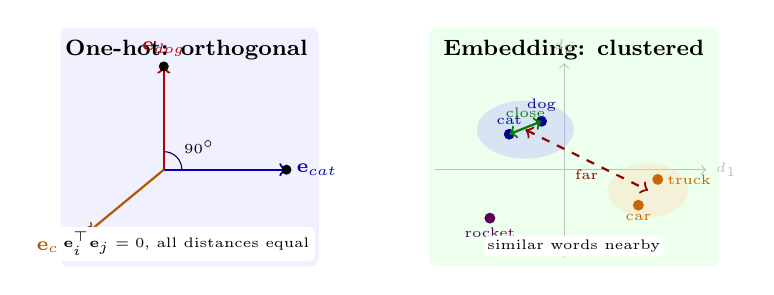
\begin{tikzpicture}[scale=0.82, every node/.style={font=\scriptsize}]
\begin{scope}
  \fill[blue!6, rounded corners=3pt] (-1.6,-1.5) rectangle (2.4,2.2);
  \node[font=\footnotesize\bfseries] at (0.35,1.85) {One-hot: orthogonal};
  \draw[->, thick, blue!70!black] (0,0)--(1.9,0) node[right] {$\mathbf{e}_{\text{cat}}$};
  \draw[->, thick, red!70!black] (0,0)--(0,1.6) node[above] {$\mathbf{e}_{\text{dog}}$};
  \draw[->, thick, orange!70!black] (0,0)--(-1.15,-0.95) node[below left] {$\mathbf{e}_{\text{car}}$};
  \foreach \p in {(1.9,0),(0,1.6),(-1.15,-0.95)} \fill \p circle (2.2pt);
  \draw[blue!40!black] (0.28,0) arc (0:90:0.28);
  \node[font=\tiny] at (0.55,0.35) {$90^{\circ}$};
  \node[font=\tiny, align=center, fill=white, rounded corners=2pt, inner sep=2pt] at (0.35,-1.15) {$\mathbf{e}_i^{\top}\mathbf{e}_j=0$, all distances equal};
\end{scope}
\begin{scope}[xshift=6.2cm]
  \fill[green!7, rounded corners=3pt] (-2.1,-1.5) rectangle (2.4,2.2);
  \node[font=\footnotesize\bfseries] at (0.15,1.85) {Embedding: clustered};
  \draw[->, thin, gray!50] (-2.0,0)--(2.2,0) node[right, font=\tiny] {$d_{1}$};
  \draw[->, thin, gray!50] (0,-1.35)--(0,1.65) node[above, font=\tiny] {$d_{2}$};
  \fill[blue!30, opacity=0.35] (-0.60,0.62) ellipse (0.75 and 0.45);
  \fill[orange!30, opacity=0.35] (1.30,-0.32) ellipse (0.62 and 0.42);
  \fill[blue!60!black] (-0.85,0.55) circle (2.4pt) node[above, font=\tiny] {cat};
  \fill[blue!60!black] (-0.35,0.75) circle (2.4pt) node[above, font=\tiny] {dog};
  \fill[orange!80!black] (1.15,-0.55) circle (2.4pt) node[below, font=\tiny] {car};
  \fill[orange!80!black] (1.45,-0.15) circle (2.4pt) node[right, font=\tiny] {truck};
  \fill[violet!70!black] (-1.15,-0.75) circle (2.4pt) node[below, font=\tiny] {rocket};
  \draw[<->, thick, green!50!black] (-0.85,0.55)--(-0.35,0.75) node[midway, above, font=\tiny] {close};
  \draw[<->, thick, red!60!black, dashed] (-0.60,0.62)--(1.30,-0.32) node[midway, below, font=\tiny] {far};
  \node[font=\tiny, fill=white, rounded corners=2pt, inner sep=1.5pt] at (0.15,-1.18) {similar words nearby};
\end{scope}
\end{tikzpicture}
\caption{Left: one-hot axes are orthogonal ($90^{\circ}$); every pair has
distance $\sqrt2$. Right: dense embeddings ($d\ll|V|$, e.g.\ $100$--$300$)
place semantically similar words nearby; distance now carries meaning.}
\label{fig:onehot-vs-embedding}
\end{figure}
\section{Distributional Hypothesis and the Embedding Matrix}
\label{sec:distributional}
\paragraph{Intuition.} Firth's hypothesis: words in similar contexts have
similar meanings. ``The \emph{cat} sat on the mat'' and ``The \emph{dog} sat
on the mat'' share the frame ``The \_\_ sat on the mat'', so cat/dog should
obtain nearby vectors. We learn vectors by making them \emph{predict} context.
\paragraph{Formal: embedding matrix.} Let $d\ll|V|$ be the embedding dimension.
Collect vectors as columns of
\begin{equation}
  \mathbf{E}\in\mathbb{R}^{d\times |V|}=[\,\mathbf{v}_{1}\;\cdots\;\mathbf{v}_{|V|}\,].
\end{equation}
If $\mathbf{x}_{i}\in\{0,1\}^{|V|}$ is the one-hot for $w_{i}$, lookup is
\begin{equation}
  \mathbf{v}_{i}=\mathbf{E}\mathbf{x}_{i}\quad\text{(selects column $i$).}
\end{equation}
Training adjusts $\mathbf{E}$ so dot products $\mathbf{v}_{i}^{\top}
\mathbf{v}_{j}$ reflect co-occurrence. Often two matrices are kept:
$\mathbf{W}\in\mathbb{R}^{|V|\times d}$ (input) and
$\mathbf{W}'\in\mathbb{R}^{d\times |V|}$ (context) with vectors
$\mathbf{v}_{w},\mathbf{v}'_{w}$. Cosine
$\cos(\mathbf{v}_{i},\mathbf{v}_{j})=\mathbf{v}_{i}^{\top}\mathbf{v}_{j}/
(\|\mathbf{v}_{i}\|\|\mathbf{v}_{j}\|)$ measures relatedness.
\section{Word2Vec: CBOW and Skip-Gram}
\label{sec:word2vec}
Word2Vec (Mikolov et al., 2013) learns $\mathbf{E}$ by self-supervision on
running text with two mirror architectures.
\paragraph{Skip-gram:} given centre $w_{I}$, predict each context $w_{O}$ in
window $c$ ($c=2$ means two left, two right). \textbf{CBOW} does the reverse:
average $2c$ context vectors to predict the centre. CBOW smooths and is
faster; skip-gram treats each context separately and handles rare words
better---hence more common on large corpora.
\begin{figure}[h]
\centering
\begin{tikzpicture}[scale=0.84, every node/.style={font=\scriptsize},
  box/.style={draw, thick, rounded corners=3pt, align=center, minimum height=0.85cm},
  arrow/.style={-{Latex}, thick}]
  \node[box, fill=blue!15, minimum width=1.85cm] (inp) at (0,0) {One-hot\\$\mathbf{x}_{w_I}$};
  \node[box, fill=green!18, minimum width=1.85cm] (emb) at (3.15,0) {Embedding\\$\mathbf{h}=\mathbf{W}^{\top}\mathbf{x}_{w_I}$\\$\in\mathbb{R}^{d}$};
  \node[box, fill=orange!18, minimum width=1.85cm] (score) at (6.3,0) {Scores\\$\mathbf{u}=\mathbf{W}'^{\top}\mathbf{h}$\\$\in\mathbb{R}^{|V|}$};
  \node[box, fill=violet!15, minimum width=1.85cm] (soft) at (9.15,0) {Softmax\\$p(w_O\!\mid\! w_I)$};
  \draw[arrow, blue!60!black] (inp)--(emb) node[midway, above, font=\tiny] {$\mathbf{W}$};
  \draw[arrow, green!50!black] (emb)--(score) node[midway, above, font=\tiny] {$\mathbf{W}'$};
  \draw[arrow, orange!60!black] (score)--(soft);
  \node[font=\tiny, align=center] at (9.15,-1.15) {predict each $w_{I+j}$, $j\in[-c,c]\setminus\{0\}$};
  \draw[arrow, violet!60!black, dashed] (soft)--(9.15,-0.80);
  \node[font=\tiny, fill=yellow!12, rounded corners=2pt, inner sep=2pt] at (3.15,1.15) {$d\ll|V|$, hidden = embedding};
  \node[font=\tiny, fill=red!8, rounded corners=2pt, inner sep=2pt] at (6.3,1.15) {$|V|$ scores, expensive!};
\end{tikzpicture}
\caption{Skip-gram architecture. One-hot selects a $d$-dimensional hidden
vector; the output layer scores all $|V|$ words. CBOW reverses the arrows:
average $2c$ context embeddings to predict the centre.}
\label{fig:skipgram-arch}
\end{figure}
\paragraph{Skip-gram objective (softmax).} For corpus $w_{1},\dots,w_{T}$,
\begin{equation}
  J(\theta)=\frac{1}{T}\sum_{t=1}^{T}\sum_{\substack{-c\le j\le c\\j\neq0}}
  \log p(w_{t+j}\mid w_{t}),\quad
  p(w_{O}\mid w_{I})=\frac{\exp({\mathbf{v}'_{w_{O}}}^{\top}\mathbf{v}_{w_{I}})}
  {\sum_{w=1}^{|V|}\exp({\mathbf{v}'_{w}}^{\top}\mathbf{v}_{w_{I}})}.
  \label{eq:skipgram-softmax}
\end{equation}
The denominator sums over $|V|$ ($10^{5}$--$10^{6}$) per step---prohibitive.
\paragraph{Negative sampling.} Replace softmax by $k$ binary decisions. For
true pair $(w_{I},w_{O})$ and $k$ noise words $w_{i}\sim P_{n}(w)$
(unigram$^{3/4}$),
\begin{equation}
  J_{\textsc{neg}}=\log\sigma({\mathbf{v}'_{w_{O}}}^{\top}\mathbf{v}_{w_{I}})
  +\sum_{i=1}^{k}\mathbb{E}_{w_{i}\sim P_{n}}[\log\sigma(-{\mathbf{v}'_{w_{i}}}^{\top}\mathbf{v}_{w_{I}})],
  \label{eq:neg-sampling}
\end{equation}
where $\sigma(x)=1/(1+e^{-x})$. Cost drops to $O(k)$ with $k=5$--$20$; the
objective pulls true pairs together and pushes noise pairs apart. CBOW uses
$\bar{\mathbf{v}}=\frac1{2c}\sum_{j}\mathbf{v}_{w_{t+j}}$ in place of
$\mathbf{v}_{w_{I}}$.
\section{GloVe: Global Vectors via Weighted Least Squares}
\label{sec:glove}
Word2Vec scans local windows; GloVe (Pennington et al., 2014) exploits global
co-occurrence $X_{ij}$ = times $w_{j}$ occurs in the context of $w_{i}$.
\paragraph{Idea.} Ratios of co-occurrence probabilities carry meaning. With
$P(k\mid\text{ice})$ vs.\ $P(k\mid\text{steam})$, $k=\text{solid}$ gives ratio
$\gg1$, $k=\text{gas}$ the opposite, $k=\text{water}\approx1$. GloVe fits
\begin{equation}
  \mathbf{w}_{i}^{\top}\tilde{\mathbf{w}}_{j}+b_{i}+\tilde b_{j}\approx\log X_{ij},
\end{equation}
with word/context vectors $\mathbf{w}_{i},\tilde{\mathbf{w}}_{j}\in\mathbb{R}^{d}$
and biases $b_{i},\tilde b_{j}$.
\paragraph{Objective.} Weighted least squares over $X_{ij}>0$:
\begin{equation}
  J_{\textsc{glove}}=\sum_{i,j=1}^{|V|} f(X_{ij})
  \bigl(\mathbf{w}_{i}^{\top}\tilde{\mathbf{w}}_{j}+b_{i}+\tilde b_{j}-\log X_{ij}\bigr)^{2},
  \label{eq:glove}
\end{equation}
\begin{equation}
  f(x)=\begin{cases}(x/x_{\max})^{\alpha}&x<x_{\max}\\1&\text{otherwise}\end{cases}
  \!\!\!,\;\alpha=0.75,\;x_{\max}=100.
\end{equation}
$f$ down-weights ultra-frequent pairs (``the'') and rare noise. The sum is
over the sparse co-occurrence matrix, trainable with AdaGrad; final vector is
often $\mathbf{w}_{i}+\tilde{\mathbf{w}}_{i}$.
\section{Vector Arithmetic and Analogies}
\label{sec:analogies}
Well-trained embeddings show \emph{linear} analogy structure, e.g.
$\mathbf{v}_{\text{king}}-\mathbf{v}_{\text{man}}+\mathbf{v}_{\text{woman}}
\approx\mathbf{v}_{\text{queen}}$: one direction encodes gender, another
royalty. Analogies are tested via
\begin{equation}
  w^{*}=\arg\max_{w}\cos(\mathbf{v}_{w},\mathbf{v}_{b}-\mathbf{v}_{a}+\mathbf{v}_{c})
  \quad\text{for }a\!:\!b::c\!:\!?\;.
\end{equation}
\begin{figure}[h]
\centering
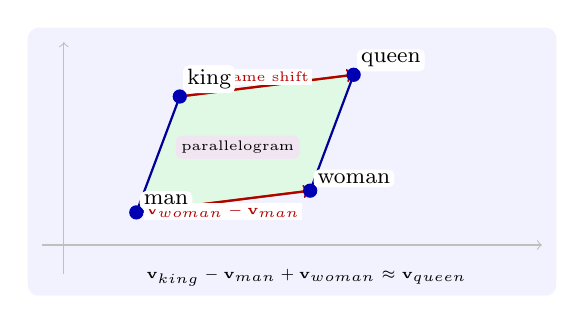
\begin{tikzpicture}[scale=0.92, every node/.style={font=\scriptsize}]
  \fill[blue!5, rounded corners=4pt] (-0.5,-0.7) rectangle (6.8,3.0);
  \draw[->, thin, gray!50] (-0.3,0)--(6.6,0); \draw[->, thin, gray!50] (0,-0.4)--(0,2.8);
  \coordinate (man) at (1.0,0.45); \coordinate (woman) at (3.4,0.75);
  \coordinate (king) at (1.6,2.05); \coordinate (queen) at (4.0,2.35);
  \fill[green!18, opacity=0.55] (man)--(king)--(queen)--(woman)--cycle;
  \draw[thick, blue!60!black] (man)--(king); \draw[thick, blue!60!black] (woman)--(queen);
  \draw[thick, orange!70!black] (man)--(woman); \draw[thick, orange!70!black] (king)--(queen);
  \draw[->, thick, red!70!black] (man)--(woman) node[midway, below, font=\tiny, fill=white, inner sep=1pt] {$\mathbf{v}_{\text{woman}}-\mathbf{v}_{\text{man}}$};
  \draw[->, thick, red!70!black] (king)--(queen) node[midway, above, font=\tiny, fill=white, inner sep=1pt] {same shift};
  \foreach \p/\lbl in {man/man, woman/woman, king/king, queen/queen} {\fill[blue!70!black] (\p) circle (2.8pt); \node[font=\footnotesize, fill=white, rounded corners=2pt, inner sep=1.5pt] at (\p) [above right=1pt] {\lbl};}
  \node[font=\tiny, fill=violet!10, rounded corners=2pt, inner sep=2pt] at (2.4,1.35) {parallelogram};
  \node[font=\tiny, align=center] at (3.35,-0.45) {$\mathbf{v}_{\text{king}}-\mathbf{v}_{\text{man}}+\mathbf{v}_{\text{woman}}\approx\mathbf{v}_{\text{queen}}$};
\end{tikzpicture}
\caption{Vector analogy as a parallelogram. The gender direction
$\mathbf{v}_{\text{woman}}-\mathbf{v}_{\text{man}}$ translates king to queen;
closure shows the relation is approximately linear (not exact---quality
depends on corpus and frequency).}
\label{fig:analogy-parallelogram}
\end{figure}
Cosine underlies nearest-neighbour search and retrieval. Analogies are
diagnostic, not definitional; contextual embeddings (Ch.~7) refine this.
\section{From Scratch in Python}
\label{sec:code-embeddings}
\begin{lstlisting}[language=Python]
import numpy as np
vocab = ["cat","dog","car","truck","rocket"]
V, d = len(vocab), 4
word_to_id = {w:i for i,w in enumerate(vocab)}
def one_hot(word):
    v = np.zeros(V); v[word_to_id[word]] = 1.0; return v
E = np.random.randn(d, V) * 0.1          # d x V embedding matrix
def embed(word):
    return E @ one_hot(word)              # selects column -> R^d
print("cat ->", embed("cat"))
def sigmoid(x): return 1/(1+np.exp(-x))
def skipgram_neg_loss(center, outside, negatives, W, Wp):
    """W: V x d, Wp: d x V; negative-sampling loss for one pair."""
    v_c = W[word_to_id[center]]
    u_o = Wp[:, word_to_id[outside]]
    loss = -np.log(sigmoid(u_o @ v_c))
    for neg in negatives:                 # push noise apart
        u_k = Wp[:, word_to_id[neg]]
        loss -= np.log(sigmoid(-u_k @ v_c))
    return loss
# gensim-style training sketch:
# W,Wp = np.random.randn(V,d)*0.01, np.random.randn(d,V)*0.01
# for center, ctx in windows(corpus, c=2):
#     negs = sample_noise(k=5, dist="unigram^0.75")
#     loss = skipgram_neg_loss(center, ctx, negs, W, Wp)
#     sgd_step(W, Wp, lr=0.025)  # + subsampling of frequent words
\end{lstlisting}
\section{Chapter Notes}
GloVe and Word2Vec unify count-based and prediction-based views; Levy \&
Goldberg (2014) show skip-gram with negative sampling implicitly factorises a
shifted PMI matrix. For code, \texttt{gensim.models.Word2Vec} handles
streaming/subsampling; see Mikolov et al.\ (2013) and Pennington et al.\
(2014) for original objectives.
\section{Exercises}
\label{sec:ch02-exercises}
\begin{enumerate}[label=E2.\arabic*, leftmargin=*, itemsep=0.7em]
    \item \textbf{One-hot geometry.} $|V|=10\,000$, $d=100$. (a) Parameters in
    $\mathbf{E}\in\mathbb{R}^{d\times|V|}$? (b) Show distinct one-hots have
    Euclidean distance $\sqrt2$ and cosine $0$. (c) Why is nearest-neighbour
    meaningless under one-hot?
    \item \textbf{Skip-gram cost.} $|V|=100\,000$, $d=300$. Estimate FLOPs for
    one forward pass of Eq.~\eqref{eq:skipgram-softmax}. With $k=10$ negatives,
    what is cost of Eq.~\eqref{eq:neg-sampling}? Explain $O(|V|)\to O(k)$.
    \item \textbf{CBOW vs.\ skip-gram.} A corpus has many rare medical terms.
    Which model gives better rare-word vectors and why? What does averaging
    $2c$ context vectors in CBOW do to gradient variance and to rare-word
    sensitivity?
    \item \textbf{GloVe weighting.} Sketch $f(x)=(x/100)^{0.75}$ for
    $0\le x\le200$. Why cap at $1$ for $x\ge100$ and use $\alpha=0.75<1$?
    What fails if $f(x)=1$ uniformly or $f(x)=x$?
    \item \textbf{Analogy arithmetic.} With pretrained GloVe 50d
    (\texttt{gensim}), test $\text{king}-\text{man}+\text{woman}\approx\text{queen}$
    via cosine. Report top-3 neighbours and one \emph{failed} analogy
    (morphological/polysemous). Why do static embeddings fail on polysemy?
\end{enumerate}
% End of Chapter 2
